\chapter[Computer vision and CNN]{Computer vision and Convolutional Neural Networks}

\textbf{Computer Vision} is a field of Artificial Intelligence which aims to implement models that performs visual tasks. Some of the tasks in this field are for example: \textit{image classification}, \textit{object detection} within an image, the so-called \textit{neural style transfer} and so on. All of this tasks, for the nature of input data, involves an enormous number of features which corresponds to a huge number of parameters to learn. How we have said several times, a \textit{classical neural network} (shallow) for example, cannot perform properly and in acceptable time such a task. Just for give an idea, the number of parameters to lean can be also around a billion! For this reason \textbf{convolutional architectures}, and then \textbf{convolutional neural networks} are introduced.

\section{Convolutional Neural Networks: main ingredients}
A \textbf{Convolutional  Neural Network} (\textbf{CNN}) is made up of several parts: (i) a \textit{convolutional layer}, (ii) a \textit{pooling layer}, (iii) a \textit{fully connected layer}.

\subsection{Convolution}
This is the core building block of a CNN, here the great majority of the computation occurs; there are several levels of this type. Besides, the convolutional layers are the ones in which the network learns the main feature from the input data. In the case of images, passing through the convolutional part of the NN low level to high level features are learned. The following figure shows an example of the extracted details at different levels of the architecture:

\begin{figure}[h]
    \centering
    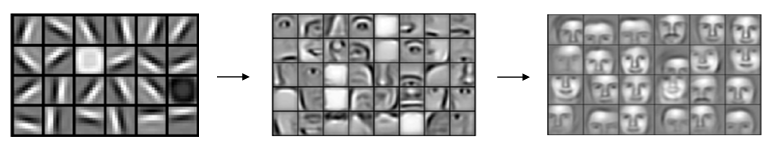
\includegraphics[scale=0.8]{img/CNN_example.png} 
\end{figure}

\noindent
You can see in the first stage only some edges are detected, passing through more complicate details arriving to the detection of entire faces. \\
This procedure takes inspiration on how our brain solve the problems; biological studies have confirmed that in order to perform a certain task, our brain solves, step by step, simpler problems in order to reach more complicate ones.\\
From now on, we are going to focus our attention on \textbf{images}, and in particular we are going deeper in some details on \textit{how convolution process works}.\\

The \textit{convolution} requires few components: (a) input data, (b) a \textbf{filter}, (c) a \textbf{feature map}. Considering that an image can be seen as a matrix of pixels, roughly speaking the filter moves across the image checking if the feature for which that filter itself has been built, is present. This process is known as \textbf{convolution}.

In the following there is a figure that shows, mathematically speaking, what are the main steps behind such a procedure.

\begin{figure}[h]
    \centering
    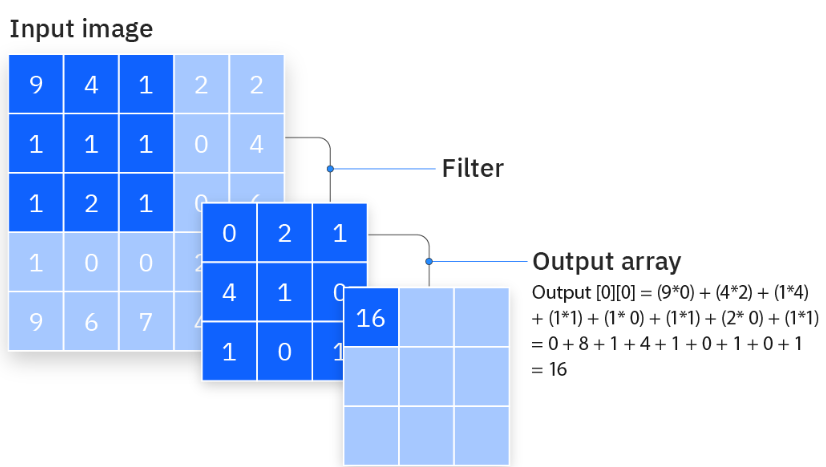
\includegraphics[scale=0.8]{img/convolution.png}
    \caption{Convolution: main steps}
\end{figure}

\noindent
In practical terms also a filter is a square matrix (with \textit{odd dimension}) in a way that it has a center. Such a filter is \textit{convolved} to the image in the sense it slides across subregions of it which have the same dimension of the feature detector; the output array (another matrix called the \textbf{feature map}) is done by scalars corresponding to the sum of the product element by element of the involved matrices. \\
How we will see, part of the parameters that the the network has to learn are those constituting such filters, then no one tells to the network how to find edges (also at different inclination) or other types of details!\\
 It should be clear that, going across the process of convolution the dimension of the matrices is reduced. In particular: starting from an image (square for simplicity) $n\times{n}$, by applying on it a filter $f\times{f}$ the dimension of the ouput will be shrinked by a quantity $f-1$ (for each dimension), with a resulting size of $(n-f+1)\times{(n-f+1)}$.

\subsubsection{Padding}
We can add a frame of padding to the image (usually by adding zeros) in order to avoid the phenomenon of \textit{shrinking dimensions}. Then, if a padding of $p$ is added to the input image (so that it results in being $(n+p)\times(n+p)$) and an $f\times{f}$ filter is applied the resulting image will have shape $(n+2p-f+1)\times{(n+2p-f+1)}$.

\begin{figure}
    \centering
    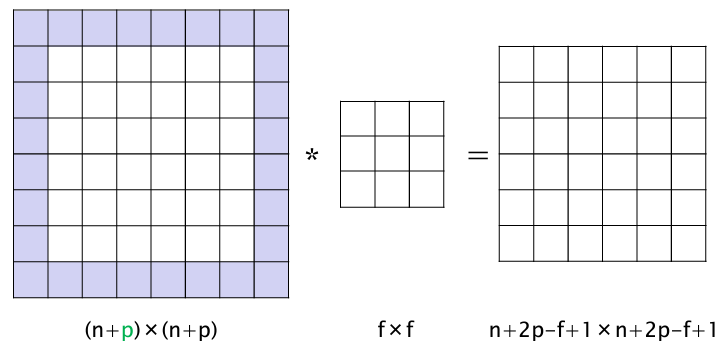
\includegraphics[scale=0.6]{img/CNN_padding.png}
    \caption{Image padding for avoiding dimension reduction}
\end{figure}

Only for a matter of nomenclature, we have to say that a convolution which does not use the padding is called \textit{valid convolution}, otherwise we have a \textit{same convolution}. The \textbf{amount of padding} to be added is such that the input and ouput images have exactly the same shape. By doing simple calculations we can find that this quantity is equal to $p=(f-1)/2$, it gives always a non-fractional value since $f$ is known to be odd.
  
\subsubsection{Strided convolutions}
The last step is needed to complete the overview on the first part of CNN: \textbf{strided convolutions}. Whether in the procedure of applying the kernel some pixels (cells of the matrix) are skipped, then the procedure is known to be \textbf{strided}. A number of skipped cells greater than one is rare, however it is remarkable that also in this case the dimension of the feature map is shrinked. More clearly, for a stride $s$ the dimensions for the output are: 
\begin{equation*}
    \left\lfloor \frac{n+2p-f}{s}+1\right\rfloor\times
    \left\lfloor \frac{n+2p-f}{s}+1\right\rfloor
\end{equation*}
How you will imagine, after some chapter of discussion on NN, such an $s$ is another hyperparameter (usually $s=1$, if a \textit{same convolution}) is used.

\subsection{Convolutions on RGB images}
In the previous paragraphs, for sake of clarity about the main aspects of convolution, we have implied that the image for which we were training the CNN was a gray-scale one. A part from few tasks, nowadays colored images are used.
Let us suppose, without loss of generality, on the contrary they are RGB ones. This implies that now the input images are not 2D-arrays anymore, they are 3D since there is an $n\times{n}$ matrix for each one of the three channels R, G, B. A \textit{3D-kernel} is needed as the number of channels. Despite the shape of the inputs is changed, what is not changing is the simple computational procedure, since all of the values are summed up! Then the feature map is always a 2D-array and the network is clearly allowed to use different or same filters. 

\subsubsection{Multiple Filters}
In the case that at this stage \textit{multiple filters} are used, also the output has a three-dimensional shape.
Now, whether on a RGB image whose shape is ${n}\times{n}\times{n_C}$, is applied $n_C'$ filters whose shape is ${f}\times{f}\times{n_C}$ (with $n_C$ being the number of channels) $\to$ the output shape will be (no padding, no striding) $(n-f+1)\times(n-f+1)\times{n_C'}$.\\

\begin{figure}[h]
    \centering
    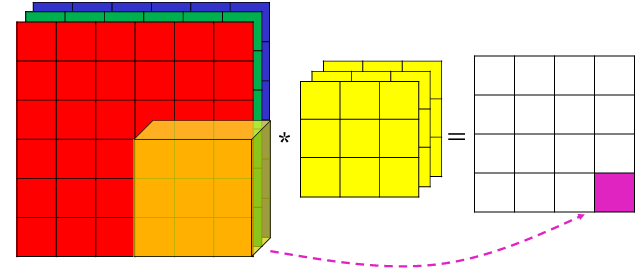
\includegraphics[scale=0.6]{img/CNN_RGB.png}
    \caption{Convolution on RGB images producing 2D-output}
\end{figure}

We can see that the convolution operation is nothing but a (just more complicated) linear combination. This is the counterpart of $z$ in the linear regression, then -- also here -- a \textit{nonlinear part} is missing! In fact, before passing the output to the next layer, even in this case an activation function is employed, in particular the ReLU. This prepares the activations for the next layer. Such a situation is well depicted in the following:

\begin{figure}[h]
    \centering
    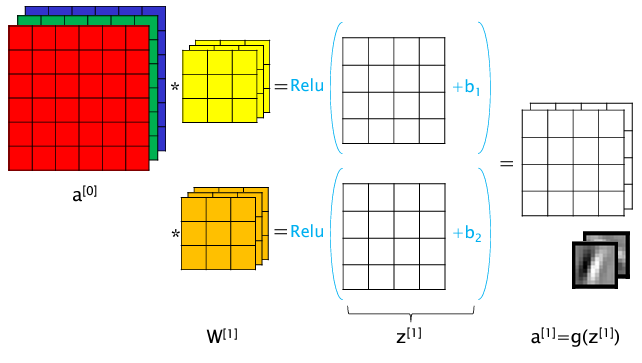
\includegraphics[scale=0.7]{img/ReLU_CNN.png}
    \caption{ReLU on feature maps}
\end{figure}